\documentclass[a4paper]{article}
\usepackage{listings}
\usepackage{geometry}
\usepackage[parfill]{parskip}
\usepackage[bottom]{footmisc}

\usepackage[bookmarks=true, bookmarksopen=true]{hyperref}
\usepackage{bookmark}
\usepackage{enumitem}
\usepackage{color}
\definecolor{linkcolour}{rgb}{0,0.2,0.6}
\hypersetup{colorlinks, breaklinks, urlcolor=linkcolour, linkcolor=linkcolour}

\usepackage{amsmath, bm}
\newcommand{\norm}[1]{\left\lVert#1\right\rVert}

\usepackage{csvsimple}

% Font
\usepackage{fontspec}
\setmainfont{GFS Artemisia}

\renewcommand{\figureautorefname}{Σχήμα}
\renewcommand{\tableautorefname}{Πίνακας}

% Images
\usepackage{graphicx}
\graphicspath{{../figures/}}
\usepackage[font={footnotesize,it}]{caption}
\usepackage[font={footnotesize}]{subcaption}
\renewcommand{\thesubfigure}{\Roman{subfigure}}
\usepackage{float}

% English-Greek use
\usepackage{polyglossia}
\setmainlanguage{greek}
\setotherlanguage{english}

% References
\usepackage[backend=biber,style=alphabetic]{biblatex}
\addbibresource{references.bib}

\geometry{
 a4paper,
 total={170mm,257mm},
 left=20mm,
 top=20mm,
}

\title{Βαθιά Μάθηση και Ανάλυση Πολυμεσικών Δεδομένων \\ Δεύτερη Εργασία}
\author{Κωστινούδης Ευάγγελος \\ΑΕΜ: 112}
\date{\today}

\begin{document}
\maketitle
\pagenumbering{gobble}
\newpage
\pagenumbering{arabic}

\section{Περιγραφή προβλήματος που επιλέχτηκε}

Για την εργασία αυτή επιλέχτηκε το πρόβλημα του super resolution. Τα δεδομένα
που χρησιμοποιήθηκαν προέρχονται από τη βάση
\href{https://data.vision.ee.ethz.ch/cvl/DIV2K/}{DIV2K}. Συγκεκριμένα,
χρησιμοποιήθηκε ένα υποσύνολο των δεδομένων αυτών.


\section{Αρχιτεκτονική μοντέλου}

Η αρχιτεκτονική του tranformer βασίζεται στην αρχιτεκτονική του Restormer
\cite{restormer}. Το δίκτυο του Restormer χρησιμοποιήθηκε για την αποκατάσταση
εικόνων και είναι πλήρων συνελικτικό.  Η αρχιτεκτονική του δικτύου παρουσιάζεται
στο παρακάτω σχήμα:

\begin{figure}[H]
    \centering

    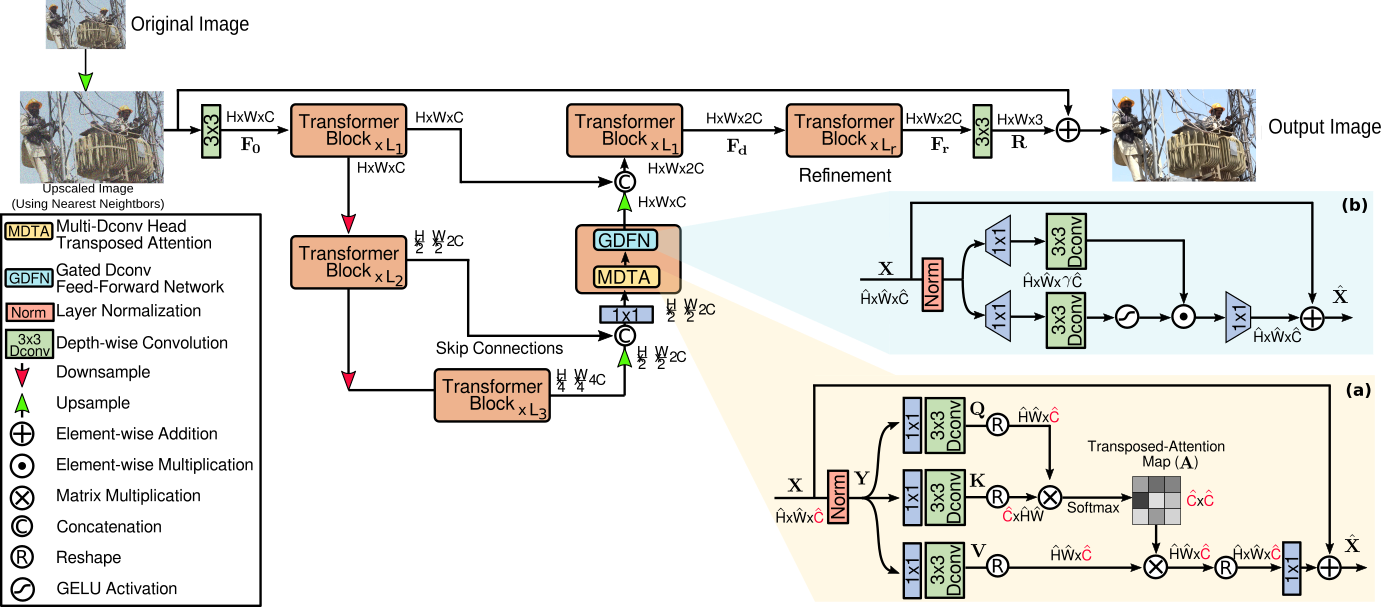
\includegraphics[width=.95\linewidth]{model.png}

    \caption{Διάγραμμα αρχιτεκτονικής δικτύου.}
    \label{fig:model}
\end{figure}

Αρχικά γίνεται υπερδειγματοληψία της εικόνα εισόδου με τη μέθοδο των
πλησιέστερων γειτόνων. Έπειτα, χρησιμοποιείται συνέλιξη με $3\times3$ kernel
ούτως ώστε, από τα 3 channels της εικόνας να γίνουν $C$ (τιμή που
χρησιμοποιήθηκε είναι $C=8$). Μετά χρησιμοποιούνται 3 επίπεδα με tranformer
blocks, όπου σε κάθε επίπεδο γίνεται υποδειγματοληψία μέσω pixel unshuffle (όταν
το επίπεδο μεγαλώνει) και υπερδειγματοληψία μέσω pixel shuffle (όταν το επίπεδο
μικραίνει). Το αποτέλεσμα που παράγουν αυτά τα επίπεδα εισέρχεται σε ένα
refinement transformer block και το αποτέλεσμα του σε συνέλιξη με $3\times3$
kernel ούτως ώστε να υπάρχουν πάλι 3 κανάλια.

To tranformer block αποτελείται από δύο κομμάτια. Το multi Dconv head transposed
attention το οποίο πραγματοποιεί τον μηχανισμό του attention μεταξύ των
καναλίων (όπως φαίνεται στο \autoref{fig:model}). Και το gated Dconv
feed-forward network.

Οι τιμές για τον αριθμό των blocks (πόσα transforer blocks υπάρχουν σε κάθε
επίπεδο) και των αριθμό των heads που χρησιμοποιήθηκαν στο τελικό δίκτυο είναι:

\begin{center}
\begin{tabular}{|c|c|c|}
\hline
Layer & Blocks \# & Heads \# \\
\hline
\hline
1     & 2        & 1       \\ \hline
2     & 2        & 2       \\ \hline
3     & 3        & 4       \\ \hline
Refinement & 2   & 1       \\ \hline
\end{tabular}
\end{center}

Ο αριθμός των παραμέτρων του δικτύου είναι 114.290.

\section{Εκπαίδευση δικτύου}

Τα δεδομένα που χρησιμοποιήθηκαν για την εκπαίδευση του δικτύου είναι οι πρώτες
100 εικόνες εκπαίδευσης της βάσης. Επίσης, για επικύρωση χρησιμοποιήθηκαν οι
πρώτες 20 εικόνες επικύρωσης της βάσης.

Για να έχουν όλες οι εικόνες το ίδιο μέγεθος, περικόπηκαν ούτως ώστε να έχουν
μέγεθος $512 \times 512$.

Ως συνάρτηση κόστους επιλέχτηκε το μέσο σφάλμα (L1 νόρμα). Το μέγεθος του batch
που χρησιμοποιήθηκε είναι 4. Το δίκτυο εκπαιδεύτηκε για 90 εποχές. Ο αλγόριθμος
βελτιστοποίησης είναι ο ADAM με ρυθμό μάθησης 0.00356. Η μέθοδος για την επιλογή
του ρυθμού μάθησης βασίζεται στο \cite{lr}. Σύμφωνα με αυτή τη μέθοδο, η
βέλτιστη τιμή του ρυθμού μάθησης δίνεται για την τιμή με μεγαλύτερη αρνητική
κλίση στο παρακάτω διάγραμμα.

\begin{figure}[H]
    \centering

    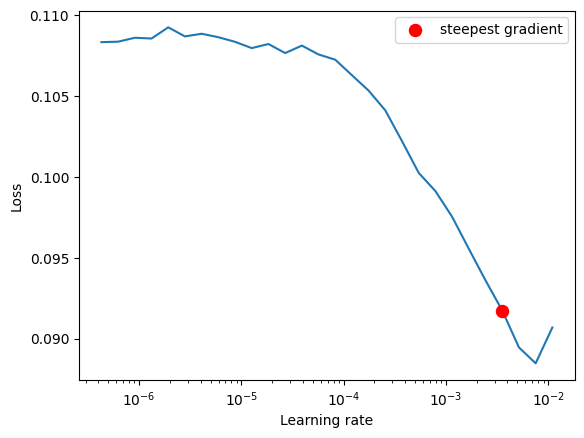
\includegraphics[width=.5\linewidth]{SRTransformer6_lr_finder.png}

    \caption{Διάγραμμα για την επιλογή του ρυθμού μάθησης.}
\end{figure}

Τα σφάλματα εκπαίδευσης του δικτύου είναι:

\begin{figure}[H]
    \centering

    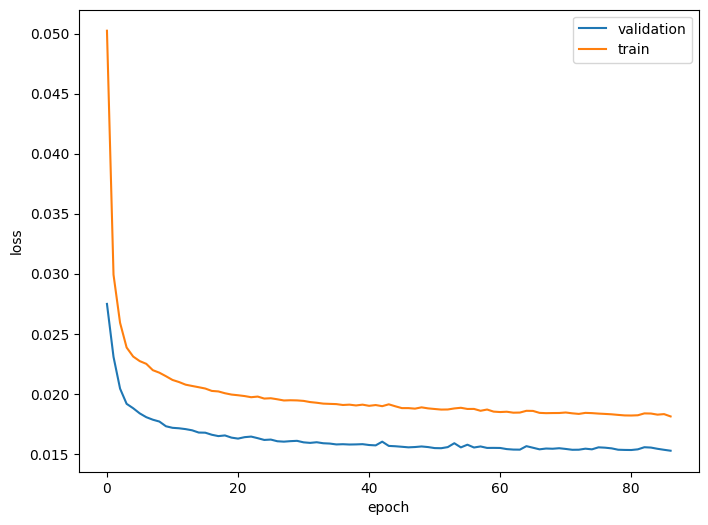
\includegraphics[width=.5\linewidth]{SRTransformer6_losses.png}

    \caption{Σφάλματα εκπαίδευσης και επικύρωσης κατά την διάρκεια της
    εκπαίδευσης.}
\end{figure}

\section{Αποτελέσματα}

Ως σύνολο ελέγχου της απόδοσης του δικτύου χρησιμοποιήθηκαν οι τελευταίες 80
εικόνες επικύρωσης της βάσης (η βάση δεν προσφέρει δεδομένα ελέγχου). Για τις
εικόνες αυτές παρουσιάζονται μετρικές για διαφορετικό μέγεθος της εικόνας
εισόδου (το δίκτυο εκπαιδεύτηκε σε εικόνες $512\time512$):

\begin{center}
\begin{tabular}{|c|c|c|c|}
\hline
\textbf{Image size} & \textbf{PSNR} & \textbf{MAE} & \textbf{MSE} \\
\hline
128  & 31.6798 & 0.020571 & 0.001465 \\ \hline
256  & 31.4181 & 0.019990 & 0.001329 \\ \hline
512  & 31.2265 & 0.019504 & 0.001252 \\ \hline
1024 & 31.9781 & 0.017348 & 0.001058 \\ \hline
\end{tabular}
\end{center}

Παρατηρούμε ότι για είσοδο $1024\time1024$ το αποτέλεσμα είναι καλύτερο για όλες
τις μετρικές. Η διαφορά μεταξύ των αποτελεσμάτων δεν είναι μεγάλη.

Στα \autoref{fig:prediction_image_128} \autoref{fig:prediction_image_256}
\autoref{fig:prediction_image_512} φαίνονται τα αποτελέσματα του μοντέλου για
διαφορετικά μεγέθη την εικόνας. Παρατηρούμε ότι η εικόνα που παράγει το
μοντέλο για όλα τα μεγέθη είναι πιο θολή. Η διαφορά αυτή παρατηρείται μόνο όταν
γίνει το ζουμάρισμα.

\begin{figure}[H]
    \centering

    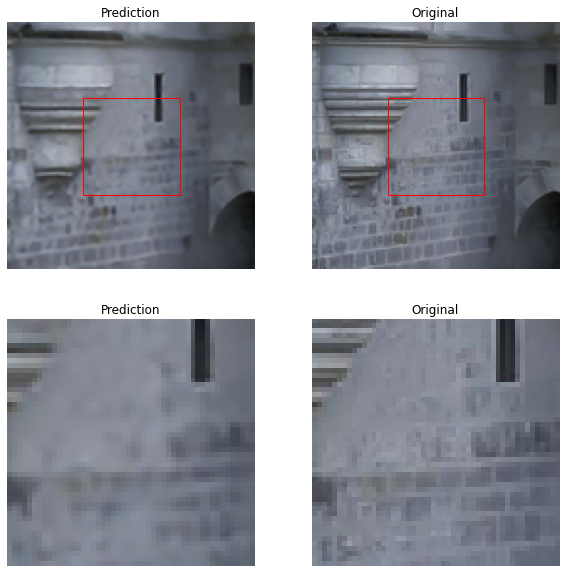
\includegraphics[width=.5\linewidth]{prediction_image_128.png}

    \caption{Αποτελέσματα μοντέλου σε μία εικόνα ελέγχου μεγέθους
    $128\times128$. Αριστερά είναι το αποτέλεσμα του μοντέλου και δεξιά η
    πραγματική εικόνα.}
    \label{fig:prediction_image_128}
\end{figure}


\begin{figure}[H]
    \centering

    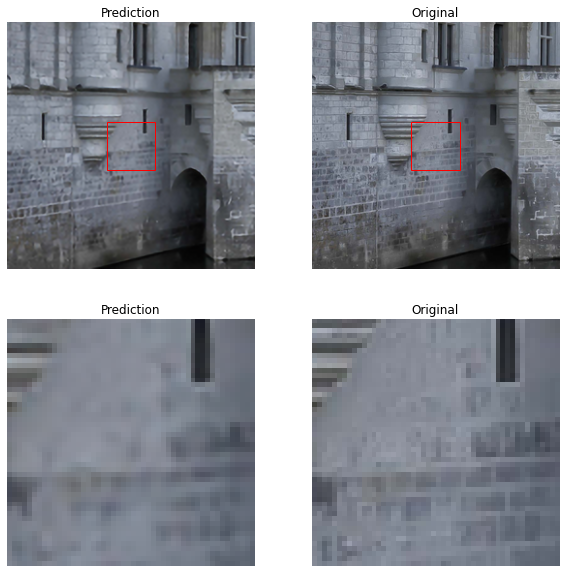
\includegraphics[width=.5\linewidth]{prediction_image_256.png}

    \caption{Αποτελέσματα μοντέλου σε μία εικόνα ελέγχου μεγέθους
    $256\times256$. Αριστερά είναι το αποτέλεσμα του μοντέλου και δεξιά η
    πραγματική εικόνα.}
    \label{fig:prediction_image_256}
\end{figure}

\begin{figure}[H]
    \centering

    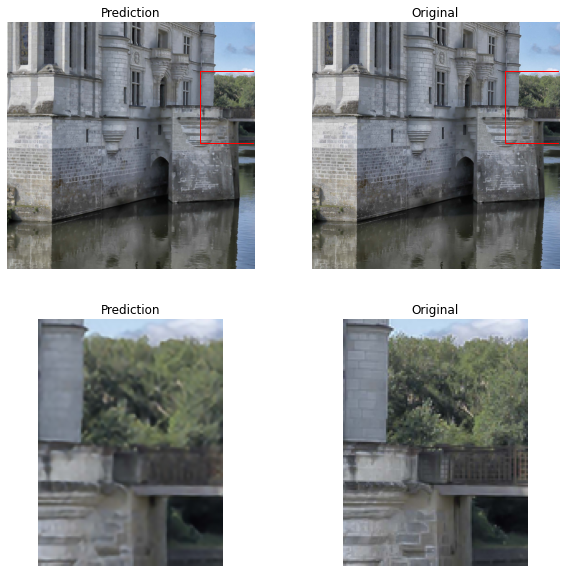
\includegraphics[width=.5\linewidth]{prediction_image_512.png}

    \caption{Αποτελέσματα μοντέλου σε μία εικόνα ελέγχου μεγέθους
    $512\times512$. Αριστερά είναι το αποτέλεσμα του μοντέλου και δεξιά η
    πραγματική εικόνα.}
    \label{fig:prediction_image_512}
\end{figure}



\newpage
\begin{english}
    \printbibliography[title=Βιβλιογραφία]
\end{english}


\end{document}
